\documentclass{article}

\usepackage[utf8]{inputenc}
\usepackage{url}
\usepackage{amsmath}
\usepackage{graphicx}
\usepackage{geometry}

\geometry{
a4paper,
left=30mm,
right=20mm,
top=30mm,
bottom=20mm,
}

\begin{document}

	\pagenumbering{gobble}
	\begin{center}

		{\LARGE Universidade Federal de Santa Catarina \par}
		\vspace {2cm}
		
		Ciências da Computação
		\vspace{2cm}

		Luca Fachini Campelli
		\vspace {4cm}

		\textbf{DESENVOLVIMENTO DE UM APLICAÇÃO PARA COLETA DE DADOS \\
				E EMISSÃO DE PASSAPORTES ELETRÔNICOS NA PLATAFORMA JAVACARD}
		\vspace {10cm}
		
		Florianópolis/SC \\

		2018
	\end{center}

	\newpage
	\begin{center}
		Luca Fachini Campelli
		\vspace{2cm}
		
		\textbf{\large DESENVOLVIMENTO DE UM APLICAÇÃO PARA COLETA DE DADOS \\
				E EMISSÃO DE PASSAPORTES ELETRÔNICOS NA PLATAFORMA JAVACARD}
		\vspace{2cm}

		\hfill \textbf{Trabalho de Conclusão de Curso \\}
		\hfill \textbf{para a graduação no curso de\\}
		\hfill \textbf{Ciências \hspace{18pt} da \hspace{18pt} Computação \\}
		\hfill \textbf{UFSC  \hspace{60pt}}

		\vspace{1cm}

		\hfill Florianópolis, 2018

	\end{center}

	\newpage

	\paragraph{\large Resumo}
		\begin{flushleft}
			\hspace{2cm} Com a preocupação com a segurança em todas as áreas, a identificação correta e segura das credenciais de uma pessoa se torna de extrema importância. A necessidade de vários documentos diferentes para as mais variadas funções faz surgir vários problemas, desde falsificação e roubo, até simples desorganização e perda.
O maior exemplo da necessidade dos mais variados documentos é em viagens internacionais. Nelas são necessárias diversas etapas até que se confirme a identidade do viajante afim de evitar falsificações, e outros tipos de ameaça, sendo o mais importante dos documentos o passaporte.\\
			\hspace{2cm} O intuito deste trabalho é criar uma infra-estrutura para emissão de passaportes eletrônicos na plataforma Javacard, baseado no padrão ICAO 9303 \cite{ICAO}, tendo em mente a segurança das informações. O sistema de emissão deverá prover um aplicativo que colete as informações do usuário, e crie um passaporte eletrônico dentro de uma das 5 possibilidades existentes e descritas no trabalho de conclusão de curso citado \cite{SASSO}.
Este cartão deve possuir todas as informações de identificação da pessoa, juntamente com informações biométricas. 
O projeto será efetuado juntamente com o LabSec (Laboratório de Segurança Computacional da UFSC) e o professor responsável, com a utilização da biblioteca JMRTD \cite{JMRTD}, que será adaptada para os fins deste projeto, e projetos anteriores do LabSec que servirão de base para desenvolvimento do produto final. \\
	\vspace{10px}
Palavras-chave: Javacard, Passaporte,JMRTD, Segurança, Passaporte-Eletrônico, e-Passport
		\end{flushleft}


	\paragraph{\large Abstract}
		\begin{flushleft}

			\hspace{2cm} With the increasing importance over security, the correct identification of a person's credentials becomes increasingly as important. The need for various documents for diferent uses brings many problems to the surface, ranging from falsification to disorganization and loss.
The greatest example being international travels, where various stages are required util the identity of an individual is confirmed, to prevent any kind of threat. The most important of these documents being the passport.\\
			\hspace{2cm} 
			This paper aims to create an infra-structure for the issuance of electronic passports on the JavaCard platform, based on the ICAO 9303 standard \cite{ICAO}, with information security in mind. The issuance system should provide an application that collects user information, and creates an electronic passport in one of 5 existing possibilities described on the cited end-term project \cite{SASSO}. This passport should posess all required user information, along with biometrics. This project will be done together with LabSec (UFSC's Computational Security Lab) and it's responsable professor, utilizing the JMRTD library \cite{JMRTD}, that shall be adapted for this project's purposes, along with prior projects from the lab, that will serve as a basis for the developing of the final product.\\

	\vspace{10px}
Key-Words: Javacard, Passaport,JMRTD, Security, Electronic-Passport, e-Passport

		\end{flushleft}
	
	\newpage

	\tableofcontents
	\newpage

	\pagenumbering{arabic}

	
	\section{Introdução}
		\begin{flushleft}
			
			\hspace{2cm}Com o aumento do compartilhamento de dados entre instituições de um mesmo grupo, a necessidade de segurança aumenta conforme o tamanho do grupo aumenta e a necessidade de confirmar a identidade de um usuário, para que não haja abuso dos recursos nem acesso irrestito aos dados se torna cada vez mais importante. Assim, cada vez mais cresce a quantidade de documentos necessários para que se confirme a identidade do usuário, como CPF, RG, CNH, Passaporte, e biometrias digitais que todos ficam armazenados em documentos físicos e separados, aumentando a quantidade de itens que uma pessoa tem que carregar, e aumentando o tempo para resgatar estas informações e conferir com o usuário. \\
			\hspace{2cm} Este trabalho visa o desenvolvimento de um sistema que controle a emissão de passaportes universitários eletrônicos baseado no padrão ICAO 9303, na plataforma Javacard \cite{JAVACHEN}. Este sistema deverá englobar todas as necessidade documentais para a identificação correta e segura do usuário, para agilizar processos de identificação biométrica. Ele deve coletar os dados do usuário como digitais, assinatura digitalizada, nome, e dados de identidade para a criação de um cartão Javacard eletrônico seguro, dentro dos vários modelos possíveis. Para tal serão utilizadas técnicas de criptografia para assegurar uma comunicação segura com o cartão, e seu funcionamento adequado. À seguir, serão discutidos alguns tópicos necessários ao entendimento destes conceitos.

			
		\end{flushleft}

	\section{O que é segurança computacional? [\cite{STALLINS} - cap 1]}
		\begin{flushleft}
			
			\hspace{2cm} Segurança computacional engloba todas as áres de pesquisa relacionadas a manter algum tipo de informação segura, seja ela uma senha, listas de cadastros, um banco de dados, documentos ou uma receita de bolo. As pesquisas relacionadas a segurança computacional, trabalham para proteger estas informaçôes de pessoas que as poderiam utilizar para maus fins, seja impedindo que elas sejam obtidas ou entendidas por outras pessoas, ou garantindo que uma informação não foi alterada antes de ser entregue ao destinatário. As próximas seções deste documento explicam certos campos desta área que serão necessários ao entendimento do leitor:
			
		\end{flushleft}

	\section{Criptografia Simétrica e Assimétrica [\cite{STALLINS} -parte 1 - parte 2]}
		\begin{flushleft}
			

 			\hspace{2cm} É possível cifrar a informação para que apenas quem possua a chave da cifra possa acessa-la. O ato de embaralhar o significado da mensagem se chama cifrar, e o inverso, decifrar. Para tal, utiliza-se algum tipo de algoritmo que, em conjunto com uma chave, seja capaz de mascarar a informação original e que seja reversível, para que com o uso da chave, se possa desfazer a criptografia e acessar o conteúdo original da mensagem. Nesta área existem dois tipos de protocolos para cifrar mensagens: a criptografia Simétrica e a Assimétrica. \\
			\hspace{2cm}Na criptografia simétrica, uma única chave é utilizada por ambas as partes, para cifrar e decifrar a mensagem. Neste contexto, as duas partes devem antecipadamente acordar a chave para ser usada entre sua comunicação. Na criptografia assimétrica, são utilizadas o que se chamam de chaves públicas e privadas. A chave pública é utilizada para cifrar, e apenas com a chave privada é possível se decifrar o conteúdo da mensagem, e vice-versa. Como o nome já diz, a chave privada é secreta, e pertence apenas a uma das partes entre as mensagens, já a chave pública é compartilhada pela rede e todos que tiverem interesse terão acesso à ela, assim, qualquer um pode enviar uma mensagem cifrada a um usuário, cifrando-a com a chave privada, e apenas o destinatário poderá lê-la. Devido às dificuldades de se utilizar este protocolo ele é mais utilizado para certiicações digitais.
					
		\end{flushleft}

	\section{Função Hash - SHA [\cite{STALLINS} - cap 11 - pg313]}
		\begin{flushleft}
			

    		\hspace{2cm} Esta função é amplamente utilizada para garantia de consistência tanto em criptografia quanto em várias outras áreas. Esta função funciona embaralhando os bits de uma mensagem à um ponto que seja impossível inverter o processo. Ela aceita uma mensagem de qualquer tamanho, porém sempre retornará uma cadeia de bytes de tamanho fixo, não importando qual seja a entrada. Porém a maior característica desta função está no fato de que para duas entradas diferentes x e y, sendo H(x) e H(y) o resultado depois de terem sido aplicados x e y respectivamente na função, nunca se deve encontrar um par tal que H(x) = H(y). Desta forma, é possível se checar a integridade de uma mensagem, aplicando a função hash sobre ela antes de ser enviada, e depois de recebida, e comparando as saídas, pois se a mensagem foi alterada, por menor que seja a alteração, os dois resultados da função serão completamente diferentes. O algoritmo mais utilizado para esta função é o SHA 2 - Secure Hash Algorithm 2(Algoritmo de Hash Seguro 2), projetado pela NSA, e possui seis versões diferentes, onde a mudança principal está no número de bits que eles retornam: SHA-224, SHA-256, SHA-384, SHA-512, SHA-512/224, SHA-512/256. 
			
		\end{flushleft}

	\section{Assinaturas Digitais[\cite{STALLINS} - cap 13.1 - pg 395]}
		\begin{flushleft}
			

			\hspace{2cm}A confiança entre duas partes de uma troca de mensagens pode não ser suficiente para que informação sensível seja transferida. Uma parte “A” pode forjar uma mensagem alegando ter sido enviada pela parte “B”, ou “B” pode simplesmente negar ter enviado qualquer mensagem, mesmo que o tenha. Desta forma, um meio de proteger âmbas as partes contra fraude mútua são as assinaturas digitais.
    Uma assinatura digital consiste em uma mensagem “M” e uma assinatura. Esta assinatura consiste de “M” passada pela função Hash explicada acima, cifrada com a chave privada do remetente e concatenada à “M”. Desta forma, para o destinatário verificar a assinatura de “M”, ele deve separar a hash cifrada de “M”, decifrá-la com a chave pública do remetente, e então comparar o resultado com “M” passado novamente pela função Hash. Se ambos os resultados forem iguais, isto provará que o remetente não poderá negar que enviou a mensagem, pois foi assinado com sua chave privada, e o destinatário não poderá forjar ou modificar a mensagem pois ele não possui a chave privada do remetente.
			
			
		\end{flushleft}


	\begin{figure}[hb!]
		\centering
		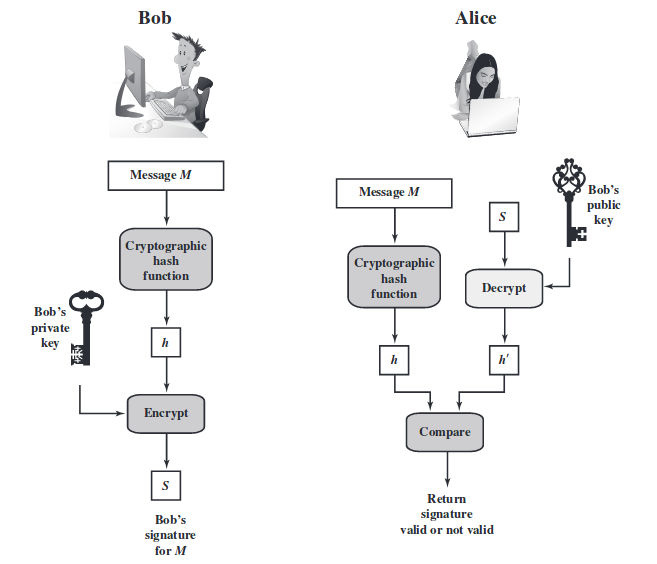
\includegraphics[width=250px]{AssinaturaDigital.png}
		\caption{Descrição simplificada do funcionamento de uma assinatura digital.}
		\label{fig:digiSign}

	\end{figure}

	\section{Certificados Digitais[\cite{STALLINS} - cap 14.4 - pg 435]}
		\begin{flushleft}
			
				
				\hspace{2cm}Certificados digitais são documentos eletrônicos que garantem a autenticidade de um certo elemento. Este que pode ser uma entidade, um site da internet ou um terminal de cartões. Um certificado é composto de algumas informações da entidade,  a chave pública da entidade, e uma assinatura digital sobre o certificado. Dependendo do tipo de certificado, esta assinatura adicionada ao final do documento é cifrada ou com a chave privada de quem o criou, denominado de certificado auto-assinado, ou com a chave privada de uma autoridade certificadora (CA - Certificate Authority). \\
				\hspace{2cm} Para que um certificado possua credibilidade, ele deve ser assinado por uma CA, e guardado em um servidor desta para que seja acessível. Para verificar a autenticidade de um certificado, deve-se separar o certificado C da hash H, decifrar a hash utilizando a chave pública da CA H’, e passar o certificado pela mesma função de hash utilizada em sua criação C’(que está incluído junto com as outras informações dentro do certificado). Se C’ for igual a H’ então pode-se confirmar que: Este certificado foi assinado pela CA e que nenhuma alteração foi feita à ele, pois como a função hash não possui duas respostas iguais para entradas diferentes, se o certificado for alterado, passando o certificado pela mesma função acarretará em uma hash diferente da que está ao final do documento, e, como ninguém mais possui a chave privada da CA, se a chave pública da CA decifrou com sucesso a hash, significa que quem a cifrou foi mesmo a CA, garantindo assim a credibilidade do certificado.

			
		\end{flushleft}

    
	\section{Javacard\cite{JAVACHEN}}
		\begin{flushleft}
			

				\hspace{2cm} O Javacard é um cartão eletrônico que possui dois componentes principais, Um chip de contato e um processador interno. Este chip de contato se faz presente do lado externo do cartão, da mesma forma que cartões de crédito ou débito modernos, e cuida da comunicação do cartão com a leitora. O processador interno funciona como um computador, ele roda um sistema operacional Java, o que torna este cartão um Javacard. Ele também possui uma memória interna capaz de armazenar dados. Este sistema operacional pode possuir aplicativos em sua memória, e dependendo do programa que os acessar, pode escolher qual deles executar. O Chip de contato fornece energia e faz a comunicação entre a leitora ou terminal e o processador.

			
		\end{flushleft}

    
	\section{O Documento ICAO 9303[1]}
		\begin{flushleft}
			
				\hspace{2cm} O documento ICAO 9303 será utilizado como base e padrão para toda formatação do aplicativo de passaporte.. ICAO é uma sigla para “International Civil Aviation Organization”, que é uma agência especializada das Nações Unidas. Foi estabelecida em 1944 para gerenciar a admnistração e governância da Convenção de Aviação Civil Internacional (Convenção de Chicago). \\
    			\hspace{2cm} O documento é escrito em 12 partes, cada uma descreve um aspecto sobre como um Passaporte Eletrônico deve ser desenvolvido, a primeira parte dando uma introdução sobre o as características de um passaporte eletrônico, e definindo siglas e acrônimos para os documentos seguintes.\\
    			\hspace{2cm} A segunda parte da especificações sobre a segurança física do cartão, desde o design interno, quanto a produção, transporte e criação do cartão. 


			
		\end{flushleft}


	\section{Estrutura Lógica de Dados - Logic Data Structure (LDS)}
		\begin{flushleft}
			
				\hspace{2cm} A estrutura lógica de dados interna do cartão se divide em 16 áreas com propósitos e formatações específicas. Sâo denominados grupos de dados (Data Groups - DG) e cada um deles armazena um tipo de informação diferente:\\
			\vspace{10px}
			\hspace{2cm} DG 1 — Informação da Zona Legível por Máquina\\
			\hspace{2cm} DG 2 — Características Faciais (Foto)\\
			\hspace{2cm} DG 3 — Informações de identificação adicionais (Digitais)*\\
			\hspace{2cm} DG 4 — Informações de identificação adicionais (Iris)*\\
			\hspace{2cm} DG 5 — Fotografia impressa na frente do cartão*\\
			\hspace{2cm} DG 6 — Reservado para uso futuro*\\
			\hspace{2cm} DG 7 — Assinatura escrita digitalizada*\\
			\hspace{2cm} DG 8 — Características de dados* **\\
			\hspace{2cm} DG 9 — Características estruturais* **\\
			\hspace{2cm} DG 10 — Características substanciais*\\
			\hspace{2cm} DG 11 — Detalhes pessoais adicionais*\\
			\hspace{2cm} DG 12 — Detalhes do documento adicionais*\\
			\hspace{2cm} DG 13 — Detalhes opcionais*\\
			\hspace{2cm} DG 14 — Informações da chave pública para Autenticação Passiva***\\
			\hspace{2cm} DG 15 — Informações da chave pública para Autenticação Ativa***\\
			\hspace{2cm} DG 16 — Pessoas para contato*\\

			\hspace{2cm} * - Opcional\\
			\hspace{2cm} ** - Ainda não definido, estrutura geral que acomoda qualquer tipo de dados\\
			\hspace{2cm} *** - Condicional, apenas se suportado\\
			\vspace{10px}
			\hspace{2cm}Além destes existem mais dois arquivos que não armazenam dados do usuário mas sim dados do cartão, estes são: COM e SOD.\\
			\hspace{2cm} O arquivo COM, ou Arquivo de Cabeçalho e de Presença de Grupos de Dados, possui a função de armazenar a presença dos arquivos de dados, ou seja, quais arquivos estão presentes no cartão, e informações de versionamento do sistema de arquivos do cartão. \\
			\hspace{2cm}O arquivo SOD, ou Document Security Object - Objeto de Segurança do Documento, possui a função de armazenar o resultado da função hash de cada arquivo, ou seja, no processo de emissão do cartão, cada arquivo é passado também pela função hash, e seu resultado é armazenado dentro do arquivo SOD. Ele também armazena todas as informações de segurança do cartão como os algoritmos utilizados para a função hash e criptografia.
		\end{flushleft}
    

	\section{Objetivos}
		\begin{flushleft}
			
				\hspace{2cm}O objetivo principal deste projeto é a criação do sistema de coleta de dados, e emissão do cartão, onde os dados sejam armazenados dentro do cartão para que depois possam ser extraídos e validados em qualquer tipo de máquina que possua este sistema.\\
				\hspace{2cm}Os objetivos específicos se dão por:\\
					\hspace{3cm}1.Coleta dos dados básicos do usuário\cite{ICAO}\cite{SASSO}\\
					\hspace{3cm}2.Coleta da foto do usuário e extração dos dados faciais da foto\cite{ISO}\cite{ICAO}.\\
					\hspace{3cm}3.Coleta dos dados biométricos como digital e íris.\\
					\hspace{3cm}4.Ter o cartão preenchido e funcional.\\
					\hspace{3cm}5.Ter o programa que colete os dados do usuário de forma rápida e fácil.\\
				 \hspace{2cm}Ao final do projeto espera-se ter concluído a criação de um sistema que colete os dados do usuário, armazenando-os no banco de dados, e que emita o cartão conforme as especificações ditadas no padrão ICAO9303

			
		\end{flushleft}

	\section{As bibliotecas utilizadas}
		\begin{flushleft}
			 
			\hspace{2cm}O sistema principal será desenvolvido na linguagem de programação Java, porém algumas das bibliotecas escolhidas foram desenvolvidas na linguagem de programação C ou C++ exigindo a utilização da Interface Nativa Java (JNI) para sua utilização.\\
		\vspace{10px}
        \hspace{2cm}JMRTD\cite{JMRTD}\\
    \hspace{2cm}Java Machine Readable Travel Documents: é uma biblioteca para a criação, edição, e aferição de passaportes eletônicos escrita na linguagem de programação Java. Ela foi desenvolvida juntamente com a biblioteca Scuba, que a complementa. Ela possui a capacidade de criar, e editar novos passaportes, além que resgatar as informações de um passaporte pronto. \\
        \vspace{10px}
		\hspace{2cm}SCUBA\cite{SCUBA}\\
    \hspace{2cm}Smart Card Utilities for Better Access: é uma biblioteca para a comunicação com cartões eletrônicos da plataforma javacard, escrita na linguagem de programação Java. Ela faz a ponte entre o JMRTD e o javacard possuindo a capacidade de transmitir mensagens e prover a comunicação com os cartões.\\
		\vspace{10px}
        \hspace{2cm}STASM\cite{STASM}\\
    \hspace{2cm}Active Shape Models with STASM: é uma biblioteca de reconhecimento facial escrita na linguagem de progrmação C++. Ela se utiliza de modelos de formas para reconhecer um rosto em uma foto e retirar os pontos de referência do rosto para que depois seja feito o reconhecimento da pessoa, fazendo uso da biblioteca Open-CV. Possui a maioria dos pontos de reconhecimento parecida com o padrão ISO\cite{ISO}, e foi escolhida por ser de fácil utilização e possuir uma extensa documentação com exemplos mínimos disponíveis, facilitando a sua compreensão, além de ser complementar à biblioteca Open-CV.\\
		\vspace{10px}
        \hspace{2cm}LIBFPRINT\cite{PRINT}\\
    \hspace{2cm}É uma biblioteca de coleção e verificação de digitais biométricas escrita na linguagem de programação C. Ela provê funções para se coletar uma digital e guardá-la como uma imagem, e depois extrair as minutas desta imagem para que se compare com uma digital recém tirada. Foi escolhida por ter uma documentação extensa, exemplos mínimos e ter sido recomendada pelo orientador deste projeto.\\
		\vspace{10px}
        \hspace{2cm}OPEN-CV\cite{OPENCV}\\
    \hspace{2cm}Open Source Computer Vision Library: é uma biblioteca para manipulação de imagens e visão computacional escrita na linguagem de programação C++ e Java. Ela possui funcionalidades para conversão de imagens, e acessar a câmera do dispositivo para tirar fotos ou videos. Ela também provê visão computacional, permitindo identificar formas e rostos na imagem. A biblioteca Stasm amplia a funcionalidade para rostos, detectando mais pontos de interesse no rosto da pessoa, e foi escolhida por ser a mais bem recomendada biblioteca de manipulação de imagens e visão computacional, com relação a sua utilização.\\
		\vspace{10px}
        \hspace{2cm}EJBCA\cite{EJBCA}\\
    \hspace{2cm}Open Source PKI Certificate Authority: é uma biblioteca para criação e manejo de certificados digitais auto-assinados escrita na linguagem de programação Java. É necessária para o funcionamento da biblioteca JMRTD, para criação dos certificados verificáveis por cartão (CVC), necessários para a execução dos protocolos de segurança do cartão.\\
		\vspace{10px}
        \hspace{2cm}BOUNCYCASTLE\cite{BOUNCYCASTLE}\\
    \hspace{2cm}Bouncy Castle Security Provider: é um provedor de segurança. É uma biblioteca que possui funções criptograficas e de geração e acordo de chaves para criptografia escrita na linguagem de programação Java. Toda a segurança da biblioteca do JMRTD é feita com ele, portanto por motivos de compatibilidade foi-se utilizado o bouncycastle como provedor para o sistema final.\\

			
		\end{flushleft}


	\section{História do Passaporte Eletrônico}
		\begin{flushleft}
			
\hspace{2cm}Quando começaram a ser utilizados, os passaportes funcionavam apenas por meio físico, na forma de uma caderneta, com todas as informações sendo verificadas manualmente, comparando as informações com o sistema. Isto acarreta em uma passagem mais lenta pelo controle e abre muitas brechas para erros e falsificações passarem pelos vigías. Várias formas de prevenir falsificações como marcas d’água foram utilizadas, porém a inovação mais impactante foi a inserção de um chip dentro do passaporte. Embora várias inforações possam ainda ser verificadas visualmente, mais ainda podem ser verificadas por meio eletrônico com o chip interno do passaporte, e mais rapidamente, diminuindo o risco de fraude. Este chip pode guardar as informações biométricas do dono, junto com as informações visuais, e ainda mais importante, possuindo diversos protocolos de segurança para garantir a autenticidade dos dados conferidos.
			
		\end{flushleft}

	\section{Metodologia}
		\begin{flushleft}
			
		\hspace{2cm}O projeto será executado tendo como base o aplicativo JMRTD\cite{JMRTD}, que engloba uma API Java e um Applet, onde juntos já permitem o armazenamento de informações no cartão, e o projeto: IDEdu: Proposta de um Cartão de Identificação Acadêmico\cite{SASSO} baseado no padrão ICAO 9303\cite{ICAO}, para que seja criado um aplicativo que emita os passaportes, e que possa ser expandido caso haja a necessidade, para englobar mais documentos e não só o passaporte.\\
		\hspace{2cm}Será feita uma extensa pesquisa sobre os documentos ICAO 9303\cite{ICAO}, e a documentação da biblioteca JMRTD para se iniciar o projeto.\\
		\hspace{2cm}O programa será desenvolvido com a linguagem de programação Java, utilizando o sistema JNI para a integração de bibliotecas que existem somente em C e C++, e as bibliotecas JMRTD, como a biblioteca principal para a construção do cartão, BouncyCastle\cite{BOUNCYCASTLE} e EJBCA\cite{EJBCA} como provedores de segurança e certificação, libfprint\cite{PRINT} para a coleta das digitais biométricas, Stasm\cite{STASM} para o reconhecimento facial, e OpenCV\cite{OPENCV} para processamento de imagem.\\
		\hspace{2cm}Utilizando uma parte do código da versão 0.4.9 da biblioteca JMRTD, é possível enviar informações para o cartão, desta forma pode-se fácilmente coletar e enviar as informações à respeito do MRZ. A biblioteca OpenCV será usada para o processamento da foto da pessoa, e possui funções para tirar a foto com a camera da máquina. Com a biblioteca Stasm, se pode retirar os pontos faciais da pessoa, e depois tratá-los para se adequarem ao padrão ICAO. Foi necessário utilizar a API nativa do java para integrar as bibliotecas Stasm e libfprint ao projeto, pois elas existem apenas em C. Com a biblioteca libfprint foi possível a extração da digital para sua inserção.

		\end{flushleft}


	\section{Os protocolos de segurança}
		\begin{flushleft}
			\hspace{2cm}Para o acesso as informações do cartão diversos protocolos de segurança devem ser efetuados para garantir a troca segura de mensagens entre o terminal e o cartão, e ter a certeza de que o terminal e o cartão não foram adulterados de alguma maneira. Todos os protocolos estão completamente descritos no documento ICAO 9303 parte 11\\
			\vspace{10px}
			\hspace{2cm} BAC - Basic Access Control - Controle de Acesso Básico\\
			\hspace{2cm} Antes de fazer qualquer tipo de operação no cartão, deve-se efetuar este protocolo. Ele utiliza as informações do número do documento, data de nascimento e de validade do cartão para criar chaves simétricas seguras para a troca de mensagens entre o terminal e o cartão. Esta informação estará impressa na frente do cartão, e portanto a execução com sucesso deste protocolo não só garante um canal de comunicação seguro, mas também confirma que as informações impressas batem com as armazenadas no cartão.\\
			\vspace{10px}
			\hspace{2cm} PA - Passive Authentication - Autenticação Passiva\\
			\hspace{2cm} Após feito o BAC, deve-se garantir a integridade estrutural de todos os dados armazenados. Assim, para isto serão utilizados os arquivos COM e SOD. Verifica-se a integridade de cada arquivo presente no cartão, indentificados pela lista de presença do arquivo COM
			
		\end{flushleft}

	\section{}
		\begin{flushleft}
			
			
		\end{flushleft}

\begingroup
	\section{Referências}
		\renewcommand{\section}[2]{}
		
		\bibliography{TCC}
		\bibliographystyle{plain}
		
\endgroup
\end{document}
